\section{Two\-Opt Class Reference}
\label{class_two_opt}\index{TwoOpt@{TwoOpt}}
Inheritance diagram for Two\-Opt::\begin{figure}[H]
\begin{center}
\leavevmode
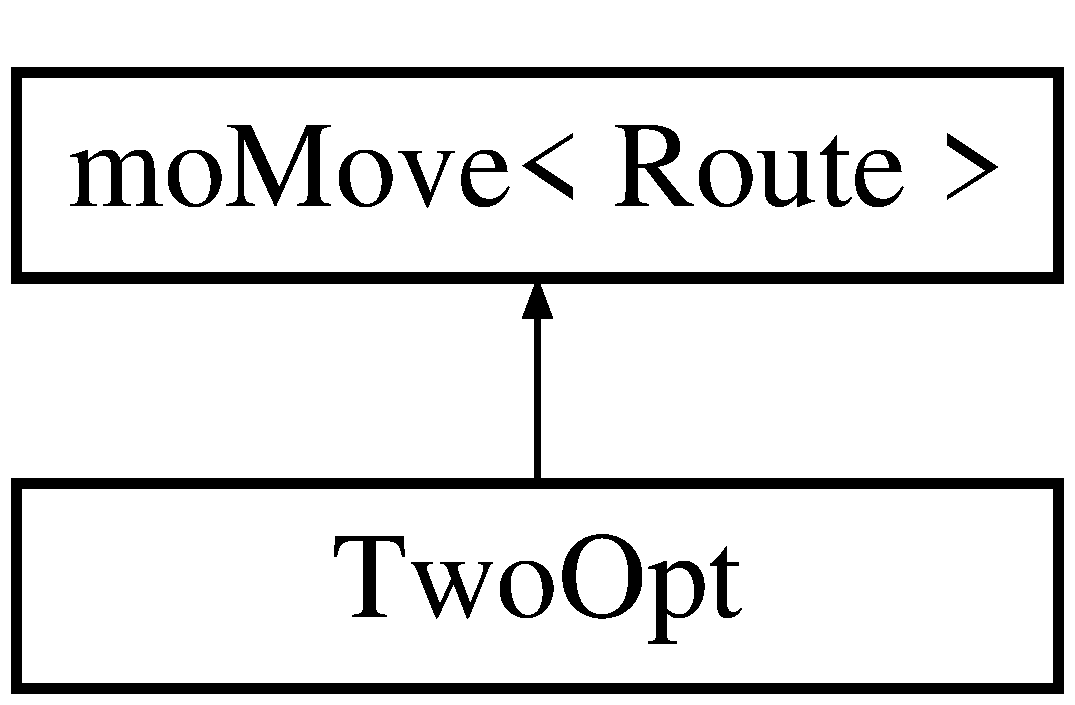
\includegraphics[height=4cm]{class_two_opt}
\end{center}
\end{figure}
\subsection*{Public Member Functions}
\begin{CompactItemize}
\item 
\bf{Two\-Opt} \bf{operator!} () const \label{class_two_opt_9fa462668a6f7293d11082d8dae26b6a}

\item 
void \bf{operator()} (\bf{Route} \&\_\-\_\-route)\label{class_two_opt_ff87d1649a33d42a6d64e8d314ed1af0}

\item 
void \bf{read\-From} (std::istream \&\_\-\_\-is)\label{class_two_opt_feccfecca2a6bd2d3a12afdf3f724be0}

\item 
void \bf{print\-On} (std::ostream \&\_\-\_\-os) const \label{class_two_opt_2400db18998b93bfb35783f6681ccd8a}

\end{CompactItemize}


\subsection{Detailed Description}




Definition at line 47 of file two\_\-opt.h.

The documentation for this class was generated from the following files:\begin{CompactItemize}
\item 
two\_\-opt.h\item 
two\_\-opt.cpp\end{CompactItemize}
